\documentclass[spanish,letterpaper,oneside]{article}

% Datos del documento
\def\documenttitle {Contextos e interacciones en el aprendizaje de las matemáticas}
\def\documentsubtitle {Fundamentos para la enseñanza y el aprendizaje I}
\def\documentsubject {Actividad 8 · Análisis bioecológico aplicado}
\def\documentauthor {Mtro. Martín Jonathan de la Cruz Muñoz}
\def\coursename {Fundamentos para la enseñanza y el aprendizaje I}
\def\coursecode {MAEM}

% Identidad institucional
\def\universityname {Instituto de Investigación, Innovación y Estudios de Posgrado para la Educación del Estado de Nuevo León}
\def\universityfaculty {Maestría en Aprendizaje y Enseñanza de las Matemáticas}
\def\universitydepartment {Fundamentos para la enseñanza y el aprendizaje I}
\def\universitydepartmentimage {img/iiiepe/marca-iiiepe.png}
\def\universitydepartmentimagecfg {height=1.75cm}
\def\universitylocation {Monterrey, Nuevo León}
\def\studentfullname {Mtro. Martín Jonathan de la Cruz Muñoz}
\def\studentid {00874}
\def\studentemail {martin.delacruz@campus.iiiepe.edu.mx}
\def\programperiod {1er tetramestre, marzo--julio de 2026}
\def\programmodality {Modalidad presencial}
\def\programshort {MAEM}

\def\authortable {
  \begin{tabular}{ll}
    \textbf{Alumno:} & \studentfullname \\
    Matrícula: & \studentid \\
    Correo institucional: & \studentemail \\
    Unidad: & \coursename \\
    Programa: & \programshort \\
    Periodo: & \programperiod \\
    & \\
    \multicolumn{2}{l}{Fecha de realización: 13 de octubre de 2026} \\
    \multicolumn{2}{l}{\universitylocation}
  \end{tabular}
}

\input{template}

\usepackage{helvet}
\renewcommand{\familydefault}{\sfdefault}
\usepackage{array}
\usepackage{longtable}
\usepackage{pdflscape}
\usepackage{tikz}
\usepackage[most]{tcolorbox}
\usetikzlibrary{arrows.meta,positioning,calc,fit,backgrounds}

\definecolor{iiiepeNavy}{HTML}{163B5C}
\definecolor{iiiepeBlue}{HTML}{1F6F9F}
\definecolor{iiiepeAqua}{HTML}{20B7A8}
\definecolor{iiiepeOrange}{HTML}{F28C28}
\definecolor{iiiepePaper}{HTML}{F6F8F7}
\definecolor{iiiepeInk}{HTML}{1E2A32}
\def\portraittitlecolor {iiiepeNavy}
\setcitestyle{authoryear,open={(},close={)}}

\newcommand{\insertcoverwatermark}{%
  \AddToShipoutPictureBG*{%
    \begin{tikzpicture}[remember picture,overlay]
      \node[opacity=.09,inner sep=0pt] at (current page.center)
      {\includegraphics[width=.58\paperwidth]{img/iiiepe/logo-puntos.png}};
    \end{tikzpicture}%
  }%
}

\newtcolorbox{reportelecturabox}[1][]{%
  enhanced,breakable,
  colback=iiiepePaper,colframe=iiiepeNavy,
  boxrule=1pt,leftrule=4pt,arc=2pt,
  left=8pt,right=8pt,top=6pt,bottom=6pt,
  before skip=6pt,after skip=10pt,
  fonttitle=\bfseries\color{white},coltitle=white,
  colbacktitle=iiiepeNavy,
  attach boxed title to top left={xshift=8pt,yshift=-2pt},
  boxed title style={colback=iiiepeNavy,colframe=iiiepeNavy,arc=1pt},
  title={Reporte de lectura},#1}

\newtcolorbox{fichalecturabox}[1][]{%
  enhanced,breakable,
  colback=iiiepeAqua!7,colframe=iiiepeAqua!70!iiiepeNavy,
  boxrule=.6pt,arc=1pt,
  left=7pt,right=7pt,top=4pt,bottom=4pt,
  fontupper=\small,before upper={\setstretch{1.0}},
  fonttitle=\bfseries\color{iiiepeNavy},coltitle=iiiepeNavy,
  colbacktitle=iiiepeAqua!7,
  title={Ficha de la lectura},#1}



\usepackage{tabularx,colortbl,pgfplots,enumitem,needspace}\pgfplotsset{compat=1.18}\definecolor{iiiepePale}{HTML}{EEF5F8}
\setlength{\parskip}{5pt}\setlength{\parindent}{0pt}
\begin{document}\insertcoverwatermark\templatePortrait\templatePagecfg\templateFinalcfg\fancyfoot{}\fancyfoot[L]{\scriptsize IIIEPE · MAEM}\fancyfoot[C]{\scriptsize\thepage}\fancyfoot[R]{\scriptsize Actividad 8}\setstretch{1.3}\raggedbottom
\section{Aprender en relaciones y contextos}
La sección del curso vincula mejoramiento del aprendizaje y teoría bioecológica de Bronfenbrenner. Este reporte desarrolla una interpretación aplicada de los sistemas ecológicos y de las interacciones que sostienen el aprendizaje. Se relacionan los sistemas ecológicos con mi docencia técnica y se distingue el contexto de las interacciones que hacen posible aprender.

\begin{center}
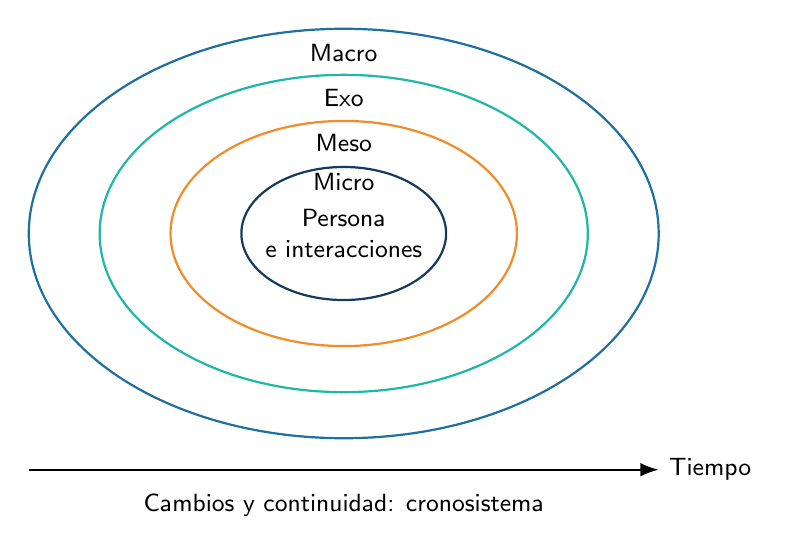
\begin{tikzpicture}[font=\small,x=1cm,y=1cm]
\foreach \r/\c in {4/iiiepeBlue,3.1/iiiepeAqua,2.2/iiiepeOrange,1.3/iiiepeNavy}\draw[\c,thick] (0,0) ellipse ({\r} and {\r*.65});
\node[align=center] at (0,0){Persona\\e interacciones};\node at (0,.65){Micro};\node at (0,1.15){Meso};\node at (0,1.72){Exo};\node at (0,2.3){Macro};\draw[-Latex,thick] (-4,-3)--(4,-3) node[right]{Tiempo};\node at (0,-3.45){Cambios y continuidad: cronosistema};\end{tikzpicture}
\end{center}
\section{Sistemas ecológicos y práctica docente}


{\small\setstretch{1.1}\renewcommand{\arraystretch}{1.25}
\begin{longtable}{|>{\raggedright\arraybackslash}p{\dimexpr0.22\linewidth-2\tabcolsep-2\arrayrulewidth\relax}|>{\raggedright\arraybackslash}p{\dimexpr0.78\linewidth-2\tabcolsep-2\arrayrulewidth\relax}|}\hline
\rowcolor{iiiepePale} \textbf{Sistema} & \textbf{Relación con el aprendizaje y decisión propuesta} \\\hline
\endfirsthead
\hline
\rowcolor{iiiepePale} \textbf{Sistema} & \textbf{Relación con el aprendizaje y decisión propuesta} \\\hline
\endhead
Microsistema & Incluye entornos de interacción directa, como aula, familia y compañeros. Una decisión es asegurar turnos de explicación, trato respetuoso y apoyo ante un error matemático. \\\hline
Mesosistema & Comprende relaciones entre microsistemas: por ejemplo, comunicación entre escuela y familia o entre espacios escolares y prácticas formativas. Propondría acuerdos comprensibles sobre tiempos y evidencias. \\\hline
Exosistema & Incluye entornos que influyen sin participación directa del estudiante, como decisiones institucionales sobre equipos o condiciones laborales de familiares. Evitaría asignar una tarea cuyo cumplimiento dependa exclusivamente de recursos no disponibles. \\\hline
\end{longtable}}



{\small\setstretch{1.1}\renewcommand{\arraystretch}{1.25}
\begin{longtable}{|>{\raggedright\arraybackslash}p{\dimexpr0.22\linewidth-2\tabcolsep-2\arrayrulewidth\relax}|>{\raggedright\arraybackslash}p{\dimexpr0.78\linewidth-2\tabcolsep-2\arrayrulewidth\relax}|}\hline
\rowcolor{iiiepePale} \textbf{Sistema} & \textbf{Relación con el aprendizaje y decisión propuesta} \\\hline
\endfirsthead
\hline
\rowcolor{iiiepePale} \textbf{Sistema} & \textbf{Relación con el aprendizaje y decisión propuesta} \\\hline
\endhead
Macrosistema & Comprende patrones culturales, valores y políticas. Analizaría expectativas sobre quién puede dominar matemáticas o tecnología y revisaría sesgos en la distribución de roles. \\\hline
Cronosistema & Considera cambios y transiciones a lo largo del tiempo. Observaría cómo se modifica una explicación entre diagnóstico, retroalimentación y transferencia, además de las transiciones de preparatoria a universidad. \\\hline
\end{longtable}}


\section{Proceso, persona, contexto y tiempo}
El modelo bioecológico no se agota en enumerar círculos. La revisión de Tong y An (2024) señala que los procesos proximales suelen recibir poca atención. Para un análisis docente, interesa qué interacciones recurrentes existen entre la persona, otras personas, objetos y símbolos, cómo cambian y en qué condiciones ocurren. No se puede deducir una causa del aprendizaje solo por ubicar un factor en un sistema.
En una secuencia de calibración, el proceso podría ser la discusión repetida de una predicción y su contraste con datos; la persona aporta saberes, intereses y recursos; el contexto incluye aula, equipo y relaciones institucionales; el tiempo comprende continuidad y revisiones. Esta mirada permite preguntar por qué un apoyo funciona para unos estudiantes y necesita ajustes para otros.
\section{Comprensión y acompañamiento}
La lectura de Sawyer incluida en el curso permite conectar el análisis con aprendizaje profundo: importa relacionar conocimientos, construir explicaciones y transferir. Mi interpretación es que un contexto técnico significativo requiere mediación; el uso de un robot no hace transparente una ecuación. Pediría predecir, representar y explicar antes de modificar parámetros.
Mi experiencia industrial ha enfatizado organización y desempeño. La perspectiva ecológica me ayuda a ampliar el diagnóstico: una entrega incompleta puede relacionarse con comprensión, acceso, tiempo o comunicación. Investigar esas condiciones no elimina la responsabilidad académica; permite definir un apoyo pertinente y un criterio claro de logro.
\section{Hipótesis de intervención y evidencias necesarias}
Una hipótesis de diseño es que la discusión recurrente de predicciones y datos puede ayudar a explicitar relaciones matemáticas. Para examinarla, distinguiría cuatro elementos: el proceso de interacción durante la tarea; los conocimientos y recursos de la persona; las oportunidades y restricciones del contexto; y la continuidad de las revisiones en el tiempo. Tong y An (2024) advierten que describir contextos no equivale a estudiar los procesos del modelo bioecológico.
El seguimiento podría conservar una explicación inicial, dos interacciones de revisión y una tarea de transferencia. Las condiciones de acceso, tiempo y participación se registrarían para interpretar diferencias sin atribuir causas automáticamente. La perspectiva ecológica orienta preguntas y apoyos; comprobar efectos requiere un diseño de observación y comparación apropiado.
El producto ofrece así una aplicación conceptual consistente con el tema de la sección. Su aportación es conectar conceptos con preguntas de intervención y evidencias que permitan revisar las decisiones docentes.

\section{Propuesta de mejora}
Propondría una tarea con alternativa digital y material, roles rotativos y un registro de revisiones. En el inicio se identifican saberes y condiciones de acceso; durante el desarrollo, preguntas breves permiten ajustar apoyos; en el cierre, cada estudiante explica un cambio. El seguimiento compara evidencias en el tiempo y evita atribuir eficacia a partir de una impresión.
La mejora esperada es una participación más distribuida y una argumentación más explícita. Son objetivos a evaluar, no resultados observados. La intervención debe revisarse a partir de las explicaciones y condiciones observadas durante su aplicación.

\needspace{5\baselineskip}\section*{Referencias}
{\setstretch{1.15}\setlength{\parskip}{6pt}
\par\hangindent=1.27cm\hangafter=1  Bronfenbrenner, U. (1987). \textit{La ecología del desarrollo humano}. Paidós.
\par\hangindent=1.27cm\hangafter=1  Sawyer, R. K. (2008). Optimizing learning: Implications of learning sciences research. En \textit{Innovating to learn, learning to innovate} (pp. 45--65). OECD. \url{https://doi.org/10.1787/9789264039958-en}
\par\hangindent=1.27cm\hangafter=1  Secretaría de Educación Pública. (2022). \textit{Plan de Estudio para la educación preescolar, primaria y secundaria}. SEP.
\par\hangindent=1.27cm\hangafter=1  Tong, P., \& An, I. S. (2024). Review of studies applying Bronfenbrenner’s bioecological theory in international and intercultural education research. \textit{Frontiers in Psychology, 14}, Article 1233925. \url{https://doi.org/10.3389/fpsyg.2023.1233925}
}

\end{document}
